%% For double-blind review submission
\documentclass[acmlarge]{acmart}\settopmatter{printfolios=true} % review will add line numbers -- anonymous will make it anonymous
%% For single-blind review submission
%\documentclass[acmlarge,review]{acmart}\settopmatter{printfolios=true}
%% For final camera-ready submission
%\documentclass[acmlarge]{acmart}\settopmatter{}
\usepackage{wrapfig}


%% Note: Authors migrating a paper from PACMPL format to traditional
%% SIGPLAN proceedings format should change 'acmlarge' to
%% 'sigplan,10pt'.

\usepackage{lipsum}  
%% Some recommended packages.
\usepackage{booktabs}   %% For formal tables:
                        %% http://ctan.org/pkg/booktabs
\usepackage{subcaption} %% For complex figures with subfigures/subcaptions
                        %% http://ctan.org/pkg/subcaption


\makeatletter\if@ACM@journal\makeatother
%% Journal information (used by PACMPL format)
%% Supplied to authors by publisher for camera-ready submission
\acmJournal{PACMPL}
\acmVolume{1}
\acmNumber{1}
\acmArticle{1}
\acmYear{2017}
\acmMonth{1}
\acmDOI{10.1145/nnnnnnn.nnnnnnn}
\startPage{1}
\else\makeatother
%% Conference information (used by SIGPLAN proceedings format)
%% Supplied to authors by publisher for camera-ready submission
\acmConference[OOPSLA'17]{The ACM SIGPLAN conference on Systems, Programming, Languages and Applications}{January 01--03, 2017}{New York, NY, USA}
\acmYear{2017}
\acmISBN{978-x-xxxx-xxxx-x/YY/MM}
\acmDOI{10.1145/nnnnnnn.nnnnnnn}
\startPage{1}
\fi


%% Copyright information
%% Supplied to authors (based on authors' rights management selection;
%% see authors.acm.org) by publisher for camera-ready submission
\setcopyright{none}             %% For review submission
%\setcopyright{acmcopyright}
%\setcopyright{acmlicensed}
%\setcopyright{rightsretained}
%\copyrightyear{2017}           %% If different from \acmYear


%% Bibliography style
\bibliographystyle{ACM-Reference-Format}
%% Citation style
%% Note: author/year citations are required for papers published as an
%% issue of PACMPL.
\citestyle{acmauthoryear}   %% For author/year citations



\begin{document}

%% Title information
\title{Why So Consistent?}         %% [Short Title] is optional;
                                        %% when present, will be used in
                                        %% header instead of Full Title.
%\titlenote{with title note}             %% \titlenote is optional;
                                        %% can be repeated if necessary;
                                        %% contents suppressed with 'anonymous'
\subtitle{Dynamic Enforcement of Fine-grained Weak Consistency}                     %% \subtitle is optional
%\subtitlenote{with subtitle note}       %% \subtitlenote is optional;
                                        %% can be repeated if necessary;
                                        %% contents suppressed with 'anonymous'


%% Author information
%% Contents and number of authors suppressed with 'anonymous'.
%% Each author should be introduced by \author, followed by
%% \authornote (optional), \orcid (optional), \affiliation, and
%% \email.
%% An author may have multiple affiliations and/or emails; repeat the
%% appropriate command.
%% Many elements are not rendered, but should be provided for metadata
%% extraction tools.

% FIRST AUTHOR
%% Author with single affiliation.
\author{Kia Rahmani}
%\authornote{with author1 note}          %% \authornote is optional;
                                        %% can be repeated if necessary
\orcid{nnnn-nnnn-nnnn-nnnn}             %% \orcid is optional
\affiliation{
  \position{PhD Student}
  \department{Computer Science}              %% \department is recommended
  \institution{Purdue University}            %% \institution is required
  \streetaddress{Street1 Address1}
  \city{City1}
  \state{State1}
  \postcode{Post-Code1}
  \country{Country1}
}
\email{rahmank@purdue.edu}          %% \email is recommended
%------------------------------------------------------------------------------------
%SECOND AUTHOR
\author{Gowtham Kaki}
%\authornote{with author1 note}          %% \authornote is optional;
                                        %% can be repeated if necessary
\orcid{nnnn-nnnn-nnnn-nnnn}             %% \orcid is optional
\affiliation{
  \position{PhD Student}
  \department{Computer Science}              %% \department is recommended
  \institution{Purdue University}            %% \institution is required
  \streetaddress{Street1 Address1}
  \city{City1}
  \state{State1}
  \postcode{Post-Code1}
  \country{Country1}
}
\email{rahmank@purdue.edu}       


%------------------------------------------------------------------------------------
%THIRD AUTHOR
\author{Suresh Jagannathan}
%\authornote{with author1 note}          %% \authornote is optional;
                                        %% can be repeated if necessary
\orcid{nnnn-nnnn-nnnn-nnnn}             %% \orcid is optional
\affiliation{
  \position{PhD Student}
  \department{Computer Science}              %% \department is recommended
  \institution{Purdue University}            %% \institution is required
  \streetaddress{Street1 Address1}
  \city{City1}
  \state{State1}
  \postcode{Post-Code1}
  \country{Country1}
}
\email{rahmank@purdue.edu}   
%------------------------------------------------------------------------------------


%% Paper note
%% The \thanks command may be used to create a "paper note" ---
%% similar to a title note or an author note, but not explicitly
%% associated with a particular element.  It will appear immediately
%% above the permission/copyright statement.
%\thanks{with paper note}                %% \thanks is optional
                                        %% can be repeated if necesary
                                        %% contents suppressed with 'anonymous'


%% Abstract
%% Note: \begin{abstract}...\end{abstract} environment must come
%% before \maketitle command
\begin{abstract}
\lipsum[1-2]
\end{abstract}


%% 2012 ACM Computing Classification System (CSS) concepts
%% Generate at 'http://dl.acm.org/ccs/ccs.cfm'.
%\begin{CCSXML}
%<ccs2012>
%<concept>
%<concept_id>10011007.10011006.10011008</concept_id>
%<concept_desc>Software and its engineering~General programming languages</concept_desc>
%<concept_significance>500</concept_significance>
%</concept>
%<concept>
%<concept_id>10003456.10003457.10003521.10003525</concept_id>
%<concept_desc>Social and professional topics~History of programming languages</concept_desc>
%<concept_significance>300</concept_significance>
%</concept>
%</ccs2012>
%\end{CCSXML}

%\ccsdesc[500]{Software and its engineering~General programming languages}
%\ccsdesc[300]{Social and professional topics~History of programming languages}
%% End of generated code


%% Keywords
%% comma separated list
%\keywords{Fine Grained Consistency , keyword2, keyword3}  %% \keywords is optional


%% \maketitle
%% Note: \maketitle command must come after title commands, author
%% commands, abstract environment, Computing Classification System
%% environment and commands, and keywords command.
\maketitle

%================================ SECTION ONE
\section{Introduction}
%\lipsum[1-13]
%================================ SECTION TWO
\section{Motivation}
%\lipsum[1-16]
%================================ SECTION THREE
\section{Related Works}
%\lipsum[1-7]
%================================ SECTION FOUR
\section{System Model}
%\lipsum[1-2]
\subsection {Overview}
%\lipsum[1-12]


\newpage
\subsection {Specification Language}
\paragraph* {} Users in our system are offered with a contract language to specify their application-level consistency requirements. 
Developers must define a contract for each operation in the application, since the overall correctness of the program requires different levels of consistency for each operation.
The constructing blocks of contracts are the relations over the set of effects generated by operations. Relations $vis(a,b)$, $so(a,b)$ and $sameobj(a,b)$ are defined to relate effects $a$ and $b$, respectively if $b$ was visible to the operation that generated $a$, if they are the result of two operations submitted by the same session, respecting their submission time, and if they were performed on the same data object.

Contracts are basically logical formulae that specify \emph{when} (the pre-condition), \emph{what} effects should be visible to an operation. For example, the Monotonic Read (MR) session guarantee, requires all the effects that are visible to an operation in a session, to be also visible to the later operations in that session. Figure \ref {fig:MR} shows how this can be succinctly defined using the relations over the effects. It simply states that all effects $\eta_s$ that satisfy the relation ($vis^{-1} (so^{-1})$) to an effect $\eta_d$, must also be visible to $\eta_d$. 
We generalized this structure and came up with blah blah


\begin{figure}
    \centering
    \begin{subfigure}[b]{0.3\textwidth}
        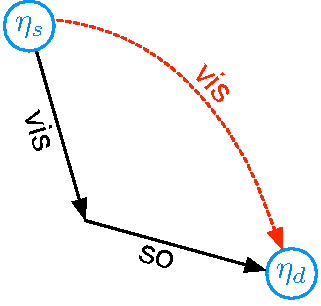
\includegraphics[width=0.66\textwidth]{../Figures/MR.pdf}
        \caption{Monotonic Read (MR)}
        \label{fig:MR}
    \end{subfigure} 
    \hspace{10 mm}
    \begin{subfigure}[b]{0.3\textwidth}
        \centering
        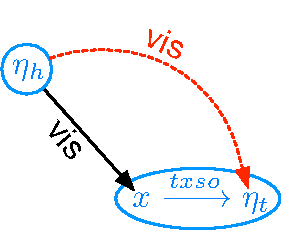
\includegraphics[width=0.66\textwidth]{../Figures/MAV.pdf}
        \caption{Monotonic Atomic View (MAV)}
        \label{fig:tMAV}
    \end{subfigure}
    \\ \hrulefill \\
    \caption{Representation of Contracts}\label{fig:contracts}
\end{figure}


\newpage
\subsection {Multi-consistent Shim}
%\lipsum[1-12]
%================================ SECTION FIVE
\section{Operational Semantics}
%\lipsum[1-2]
\subsection {Semantics of the Shim Layer}
%\lipsum[1-10]
\subsection {Semantics of the DepsFinder}
%\lipsum[1-10]
\subsection {Maximal Visibility and Minimal Wait}
%\lipsum[1-10]
%================================ SECTION SIX
\section{Implementation}
%\lipsum[1-14]
%================================ SECTION SEVEN
\section{Evaluation}
%\lipsum[1-15]
%================================ SECTION EIGHT
\section{Conclusions and Future Work}
%\lipsum[1-5]










%% Acknowledgments
%\begin{acks}                            %% acks environment is optional
                                        %% contents suppressed with 'anonymous'
  %% Commands \grantsponsor{<sponsorID>}{<name>}{<url>} and
  %% \grantnum[<url>]{<sponsorID>}{<number>} should be used to
  %% acknowledge financial support and will be used by metadata
  %% extraction tools.
%  This material is based upon work supported by the
%  \grantsponsor{GS100000001}{National Science
%    Foundation}{http://dx.doi.org/10.13039/100000001} under Grant
%  No.~\grantnum{GS100000001}{nnnnnnn} and Grant
%  No.~\grantnum{GS100000001}{mmmmmmm}.  Any opinions, findings, and
%  conclusions or recommendations expressed in this material are those
%  of the author and do not necessarily reflect the views of the
%  National Science Foundation.
%\end{acks}


%% Bibliography
%\bibliography{bibfile}


%% Appendix
%\appendix
%\section{Appendix}

%Text of appendix \ldots

\end{document}
